\section{Introduction} \label{introduction}
Human action recognition is a challenging task for computer vision algorithms due to the large variabilities in video data caused by occlusions, camera motions, actor and scene appearances, among others. A popular current trend in action recognition methods relies on using local video descriptors to represent visual events in videos \cite{laptev2005, dollar2005, wang2011}. These features are usually aggregated into a compact representation, namely the bag-of-features (BoF) representation \cite{laptev2008}. The advantage of this simple representation is that it avoids difficult pre-processing steps such as motion segmentation and tracking. In the BoF representation, local descriptors are quantized using a pre-computed codebook of visual patterns. This representation combined with discriminative classifiers such as support vector machines (SVM), has been quite successful in recognizing human actions  in controlled scenarios \cite{blank2005, schuldt2004}. Due to its simplicity, BoF requires the use of strong, robust and informative features, which can be obtained reliably in such simplified scenarios.

However, recent efforts have been made to collect more realistic video datasets (\eg from movies and personal videos uploaded to video sharing websites  \cite{kuehne2011,  marszalek2009}), which are useful for evaluating human action recognition methods in more natural settings. In fact, these datasets represent a challenge for existing BoF-based methods due to dynamic backgrounds, variations in illumination and viewpoint, and camera motion among other visual nuisances that can severely affect recognition performance. To mitigate the effect of camera motion in describing the action of interest in a video, recent methods \cite{wang2013,wang2011} have proposed using dense point trajectories in a video. In fact, these trajectories can separate background from foreground using a simple camera motion model (\ie an affine or homography transform between consecutive frames). Such separation allows action recognition approaches to robustly extract and describe foreground motion, which is otherwise contaminated by camera motion and the background. Inspired by this work, our proposed method also makes use of these dense trajectories; however, we enlist a more general camera model (by estimating the fundamental matrix between consecutive video frames) that allows for a more reliable separation between foreground and background pixels, especially in non-planar cluttered scenes. Unlike most other methods, we claim that the \emph{surrounding} of a human action, namely global camera motion and static background appearance, can also be used to discriminate between certain human actions. These surrounding cues can also be considered as contextual features for an action, which mine the relationship between the human action and both the background scene as well as the camera motion. The appearance of the scene in which an action occurs can be helpful in recognizing the action, as validated by previous work in \cite{marszalek2009}. For example, a `cooking' action tends to occur indoors, while a `jogging' action usually exists outdoors. Interestingly, the manner in which the \emph{cameraman} records a particular action can also be indicative of the action. For example, camera zoom with minimal panning usually indicates an action that is spatially limited to a smaller physical space (\eg juggling balls), while significant panning is indicative of actions that require a much larger spatial support (\eg practicing long jump). \B{We might need a more concrete example.} Our proposed approach mines these two sources of surrounding information, as well as, the separated foreground motion to describe and recognize an action. \B{We need to reference the pipeline figure too.}




\begin{figure*}[ht]
\begin{center}
%\fbox{\rule{0pt}{1in} \rule{0.9\linewidth}{0pt}}
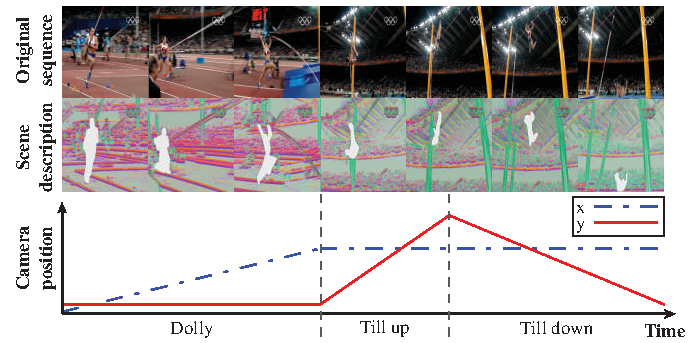
\includegraphics[width=0.98\linewidth]{fig/PullFigure.pdf}
\end{center}
\caption{Some human actions have important correlations with surrounding cues. As observed in the first row, there is a video sequence associated with the human action pole vault. It is also noticeable that the camera moves according to some specific patron for capturing the movement of the subject. Specifically, the camera moves within dolly panning tracking when the athlete is approaching the plant and take off. Then, camera slightly starts to tilling up and tilling down when the person is flying away and falling respectively. Additionally, a better description can be performed if visual appearance of the track field is captured.}
\label{fig:pull_figure}
\end{figure*}



\subsection*{Related work}\label{subsec: related work}
A large body of work has studied the problem of human action recognition in video. For a survey of this work, we refer the reader to \cite{aggarwal2011}. In this section, we give an overview of previous work that is most relevant to our proposed method.

%on the topic of feature extraction and action recognition in videos.

\paragraph{\textbf{Action Recognition Pipeline.}}The majority of action recognition methods rely on local descriptors to represent visual events in videos \cite{laptev2005,dollar2005,wang2011}. Traditionally, these features are usually aggregated into a compact representation using the bag-of-features (BoF) framework \cite{laptev2008}. Moreover, recent studies show that using soft encoding techniques, such as  Fisher Vectors \cite{perronnin2010} and Vectors of Locally Aggregated Descriptors (VLAD) \cite{jegou2012}, can lead to a boost in action recognition performance. These representations combined with discriminative classifiers such as support vector machines (SVM), have been quite successful in discriminating human action classes. However, as discussed in \cite{xwang2013}, there remain many details of the overall action recognition pipeline that can be extensively explored, including feature extraction, feature pre-procesing, codebook generation, feature encoding and pooling and normalization. In this paper, we propose a new set of features that can be used to address some of the limitations of conventional feature extraction methods.

\paragraph{\textbf{Feature Extraction.}} When applied to videos with substantial camera motion, traditional feature extraction approaches \cite{dollar2005, laptev2005} tend to generate a large number of features, which are inherently dependent on the camera motion in a video, thus, limiting their discriminative power among action classes. In order to overcome this issue, Wu \etal \cite{wu2011} propose the use of Lagrangian point trajectories for action description in videos acquired with moving cameras. Their method compensates for global camera motion and only extracts features that exhibit motion independent of the camera movement, thus, outperforming traditional feature extraction algorithms. Park \etal \cite{park2013} use a weak video stabilization method based on extracting coarse optical flow to isolate limb motion while canceling pedestrian translation and camera motion. Wang \etal \cite{wang2011} present a method for action recognition using dense sampling of point trajectories. Their method handles large camera motions by limiting the maximum length of tracked trajectories. Despite their simplicity, these dense trajectory features have been shown to achieve a significant performance improvement as compared to conventionally detecting sparse and salient spatiotemporal features \cite{laptev2005}.

More recent methods improve upon the aforementioned dense trajectory features. For example, Jain \etal \cite{jain2013} propose a method to estimate more reliable trajectory features for action recognition. This method provides additional reliability and robustness to the feature extraction stage by initially decomposing optical flow into dominant and residual motions. Dominant motion is estimated using an affine frame-to-frame motion model and is subtracted from the computed optical flow to obtain the residual motion, which is attributed to the human action of interest. Similarly, 'improved trajectories' are proposed in \cite{wang2013} to stabilize features and compensate for simple camera motion. This is done by fitting a frame-to-frame homography (using RANSAC) to separate moving points of the human action from those of the background. By explicitly modeling camera motion, their framework improves the performance of several motion descriptors, including trajectory shape, histogram of optical flow (HOF), and motion boundary histograms (MBH). While these methods have been successful in separating background/residual motions, surrounding cues of human actions are usually discarded, thus, ignoring contextual information such as the static scene appearance and distinct global motions correlated with specific actions.

Moreover, a few approaches have investigated ways to involve background contextual information in the action recognition pipeline. Marszalek \etal \cite{marszalek2009} incorporate context information from movie scripts by modeling the relationship between human actions and static scenes based on textual co-occurrence. While such textual co-occurrence helps recognition, they are restricted only to video sources where scripts are available. In \cite{ikizler2010}, multiple feature channels are integrated from different sources of information including human motion, scene information, and objects in the scene. However, this approach makes use of all pixels (corresponding to both the human action and background scene) to generate a global descriptor of the static scene \cite{oliva2001}. Rather than computing such a holistic representation, our proposed method separtely computes a scene descriptor only from the extracted background, a motion descriptor from the extracted foreground trajectories, and a camera motion descriptor from the estimated transformations between consecutive frames.

In this paper, our goal is to reliably alleviate the effect of camera motion, as well as, incorporate features describing an action's surrounding to build a richer representation for human actions. We are motivated by the fact that most videos are filmed with an intention and therefore there exists a correlation between the inherent camera motion in a video and the portrayed human action itself. We encode this intention with a weak camera motion model based on frame-to-frame fundamental matrices in a video. To the best of our knowledge, this is the first work to mine such a relationship between human actions and the filming process.








%A large amount of work has studied the problem of human action recognition in videos \cite{Aggarwal2011}. In
%this section we overview some of the most relevant previous work on the topics of video stabilization, video
%feature extraction and action recognition in videos.
%
%A common methodology for video stabilization relies on estimating the global camera motion. One approach for
%this estimation computes sparse visual features \cite{Brown2003,Capel1998, Zoghlami1997} such as corners
%\cite{Censi1999} and estimates a warping matrix between consecutive frames. Others prefer to use all pixels
%in the image to compute an alignment \cite{Lucas1981, Matsushita2006}, but tend to suffer under-fitting due
%to local outliers. An alternative methodology defines a model for camera motion
%\cite{Buehler2001,Hansen1994} and uses multiple frames to estimate its parameters. Unfortunately, there is a
%large variation in camera motions and it is difficult to capture them in a single model. Once the camera
%motion is estimated, most algorithms use it to perform image alignment or warping \cite{szeliski2006image}.
%Unfortunately, warping usually introduces empty image regions in the aligned image. These areas may be
%recovered using impainting methods \cite{Wexler2004} at a high computational cost. Finally, instead of fully
%stabilizing sequences, \cite{Gleicher2008,GrundmannKwatra2011} propose to simulate professional camera
%motion in videos taken with handheld cameras. Unfortunately, not all camera motion is removed and the
%application of these methods to action recognition is limited. Most related to our approach, Park \etal
%\cite{Park2013} recently show how the use of weak video stabilization based on a coarse optical flow can
%lead to improved pedestrian detection in videos. Their goal is to isolate limb motion while cancelling
%pedestrian translation and camera motion. In this paper, we explore the extension of this technique and its
%applicability to feature extraction for action recognition.
%In another line of work, researchers have studied the issue of extracting video features for recognition
%that are robust to camera motion \cite{Jain2013,Gross2012,Wu2011a}. When applied to videos with large camera
%movement, traditional video feature extraction methods tend to generate a large number of features that are
%mostly related to the camera motion \cite{Dollar2005, Laptev2005, WangCVPR2011}. In order to overcome this
%issue, Wu \etal \cite{Wu2011a} propose the use of Lagrangian particle trajectories for action description in
%videos acquired with moving cameras. Their method compensates for the global camera motion and only extracts
%features that exhibit motion independent to the camera movement, outperforming traditional feature
%extraction algorithms. Matikainen \etal \cite{Matikainen2009} present a technique for action recognition
%with quantized trajectories of tracked features. More recently, Wang \etal presents a method for action
%recognition using dense sampling of point trajectories \cite{WangCVPR2011}. Their method handles large
%camera motions by limiting the maximum length of tracked trajectories. In spite of their simplicity, these
%dense trajectory features achieved state-of-the-art performance in bench-marking datasets. In order to
%improve upon these dense trajectories, Jain \etal \cite{Jain2013} propose a method to estimate more reliable
%motion features for action recognition. Their method obtains improvements on feature robustness  by first
%decomposing optical flow into dominant and residual motions. Dominant motion is estimated using an affine
%model and subtracted from the computed optical flow to obtain the residual motion. This information is then
%used to compute local motion descriptors. While the method is simple and improves recognition performance,
%residual and dominant motion estimations are not reliable when the dominant motion is related to the actor.
